\documentclass[UTF8,12pt,AutoFakeBold=2]{ctexart}

\RequirePackage{
    nsfc,
    amsmath,
    graphicx,
    siunitx,
    booktabs,
    multirow,
    rotating
}

\begin{document}

\SetTitle{报告正文}
\TitleDes{参照以下提纲撰写,要求内容翔实、清晰,层次分明,标题突出。}{请勿删除或改动下述提纲标题及括号中的文字。}

\ContentDes{(一)立项依据与研究内容}{(建议8000字以下):}

\NsfcSection{1}{项目的立项依据}{
(研究意义、国内外研究现状及发展动态分析,需结合科学研究发展趋势来论述科学意义;或结合国民经济和社会发展中迫切需要解决的关键科技问题来论述其应用前景。附主要参考文献目录);}

\subsection{研究意义}

Lorem Ipsum是一种常用的虚拟填充文本,在网页设计和排版领域有着广泛的应用。它的历史可以追溯到16世纪,最初被用作印刷业的占位符文本。Lorem Ipsum文本并非无意义的乱码,而是源自古罗马时期的拉丁文文献。经过几个世纪的发展,这段文本逐渐演变成了一种标准化的虚拟填充文本,被广泛应用于各种设计项目中\cite{iijima1991helical}。

Lorem Ipsum之所以能够经久不衰,一方面是因为其本身的可读性和连贯性,另一方面则得益于它能够有效地模拟真实文本的视觉效果,帮助设计师们更好地预览最终的设计成果。\textbf{随着数字时代的发展,Lorem Ipsum也逐渐从传统的印刷领域扩展到了网页设计、移动应用等多个领域,成为了设计师们不可或缺的工具之一}\cite{iijima1991helical, aharony2000large, susskind1995world, kitaev2003fault}。

\subsection{国内外研究现状及发展动态分析}

\subsubsection{XXX的研究现状}

各类方法之间的对比详见表\ref{tab:comparison}。

\begin{sidewaystable}
	\caption{\label{tab:comparison}各种XXX方法的参数对比}
	\centering
	\begin{tabular}{cccccccc}
		\toprule
		\textbf{方法}	&	\textbf{设备}	&	\textbf{参数1}	&	\textbf{参数2}	&	\textbf{参数3}	&	\textbf{参数4} 	&	\textbf{参数5}	&	\textbf{参数6} \\
		\midrule
		\multirow{12}{*}{\textbf{方法1}} & 设备1\cite{iijima1991helical} & XXX & --- & --- & --- & \textasciitilde\SI{1}{\um} & --- \\
		& 设备2\cite{lowry1951protein} & XXX & --- & --- & --- & \textasciitilde\SI{1}{\um} & --- \\
		& 设备3\cite{bradford1976rapid, einstein1935can, randall1999alternative} & XXX & --- & --- & --- & \textasciitilde\SI{1}{\um} & --- \\
		& 设备4\cite{laemmli1970cleavage} & XXX & --- & --- & --- & \textasciitilde\SI{1}{\um} & --- \\
		& 设备5\cite{maldacena1999large} & XXX & --- & --- & --- & \textasciitilde\SI{1}{\um} & --- \\
		& 设备6\cite{gubser1998gauge} & XXX & --- & --- & --- & \textasciitilde\SI{1}{\um} & --- \\
		& 设备7\cite{randall1999alternative} & XXX & --- & --- & --- & \textasciitilde\SI{1}{\um} & --- \\
		& 设备8\cite{aharony2000large} & XXX & --- & --- & --- & \textasciitilde\SI{1}{\um} & --- \\
		& 设备9\cite{copeland2006dynamics} & XXX & --- & --- & --- & \textasciitilde\SI{1}{\um} & --- \\
		& 设备10\cite{susskind1995world} & XXX & --- & --- & --- & \textasciitilde\SI{1}{\um} & --- \\
		& 设备11\cite{kitaev2003fault} & XXX & --- & --- & --- & \textasciitilde\SI{1}{\um} & --- \\
		& 设备12\cite{breiman2001random} & XXX & --- & --- & --- & \textasciitilde\SI{1}{\um} & --- \\
		\textbf{方法2} & 设备13\cite{pedregosa2011scikit} & XXX & --- & --- & --- & \textasciitilde\SI{1}{\um} & --- \\
		\bottomrule
	\end{tabular}
\end{sidewaystable}



\subsubsection{XXX的研究现状}

申请人前期做了XXX\cite{zhang2024one, zhang2024another}。

\subsection{本项目的创新思维}


\bibliography{references}

\NsfcSection{2}{项目的研究内容、研究目标,以及拟解决的关键科学问题}{
(此部分为重点阐述内容);}

\subsection{研究目标}

Lorem Ipsum是一种常用的虚拟填充文本,在网页设计和排版领域有着广泛的应用。它的历史可以追溯到16世纪,最初被用作印刷业的占位符文本。Lorem Ipsum文本并非无意义的乱码,而是源自古罗马时期的拉丁文文献。经过几个世纪的发展,这段文本逐渐演变成了一种标准化的虚拟填充文本,被广泛应用于各种设计项目中。

Lorem Ipsum之所以能够经久不衰,一方面是因为其本身的可读性和连贯性,另一方面则得益于它能够有效地模拟真实文本的视觉效果,帮助设计师们更好地预览最终的设计成果。随着数字时代的发展,Lorem Ipsum也逐渐从传统的印刷领域扩展到了网页设计、移动应用等多个领域,成为了设计师们不可或缺的工具之一。

\subsection{研究内容}

\subsubsection*{(1) 研究内容一}

\subsubsection*{(2) 研究内容二}

\subsubsection*{(3) 研究内容三}

\subsection{拟解决的关键科学问题}
\subsubsection*{(1) 关键科学问题一}

\subsubsection*{(2) 关键科学问题二}

\NsfcSection{3}{拟采取的研究方案及可行性分析}{
(包括研究方法、技术路线、实验手段、关键技术等说明);}

\subsection{研究方案}

\subsubsection{研究内容一}

\subsubsection{研究内容二}

\subsubsection{研究内容三}

\subsection{拟采用技术路线}

本项目所采用的总体技术路线如图\ref{fig:roadmap}所示。
\begin{figure}[htbp]
	\centering
	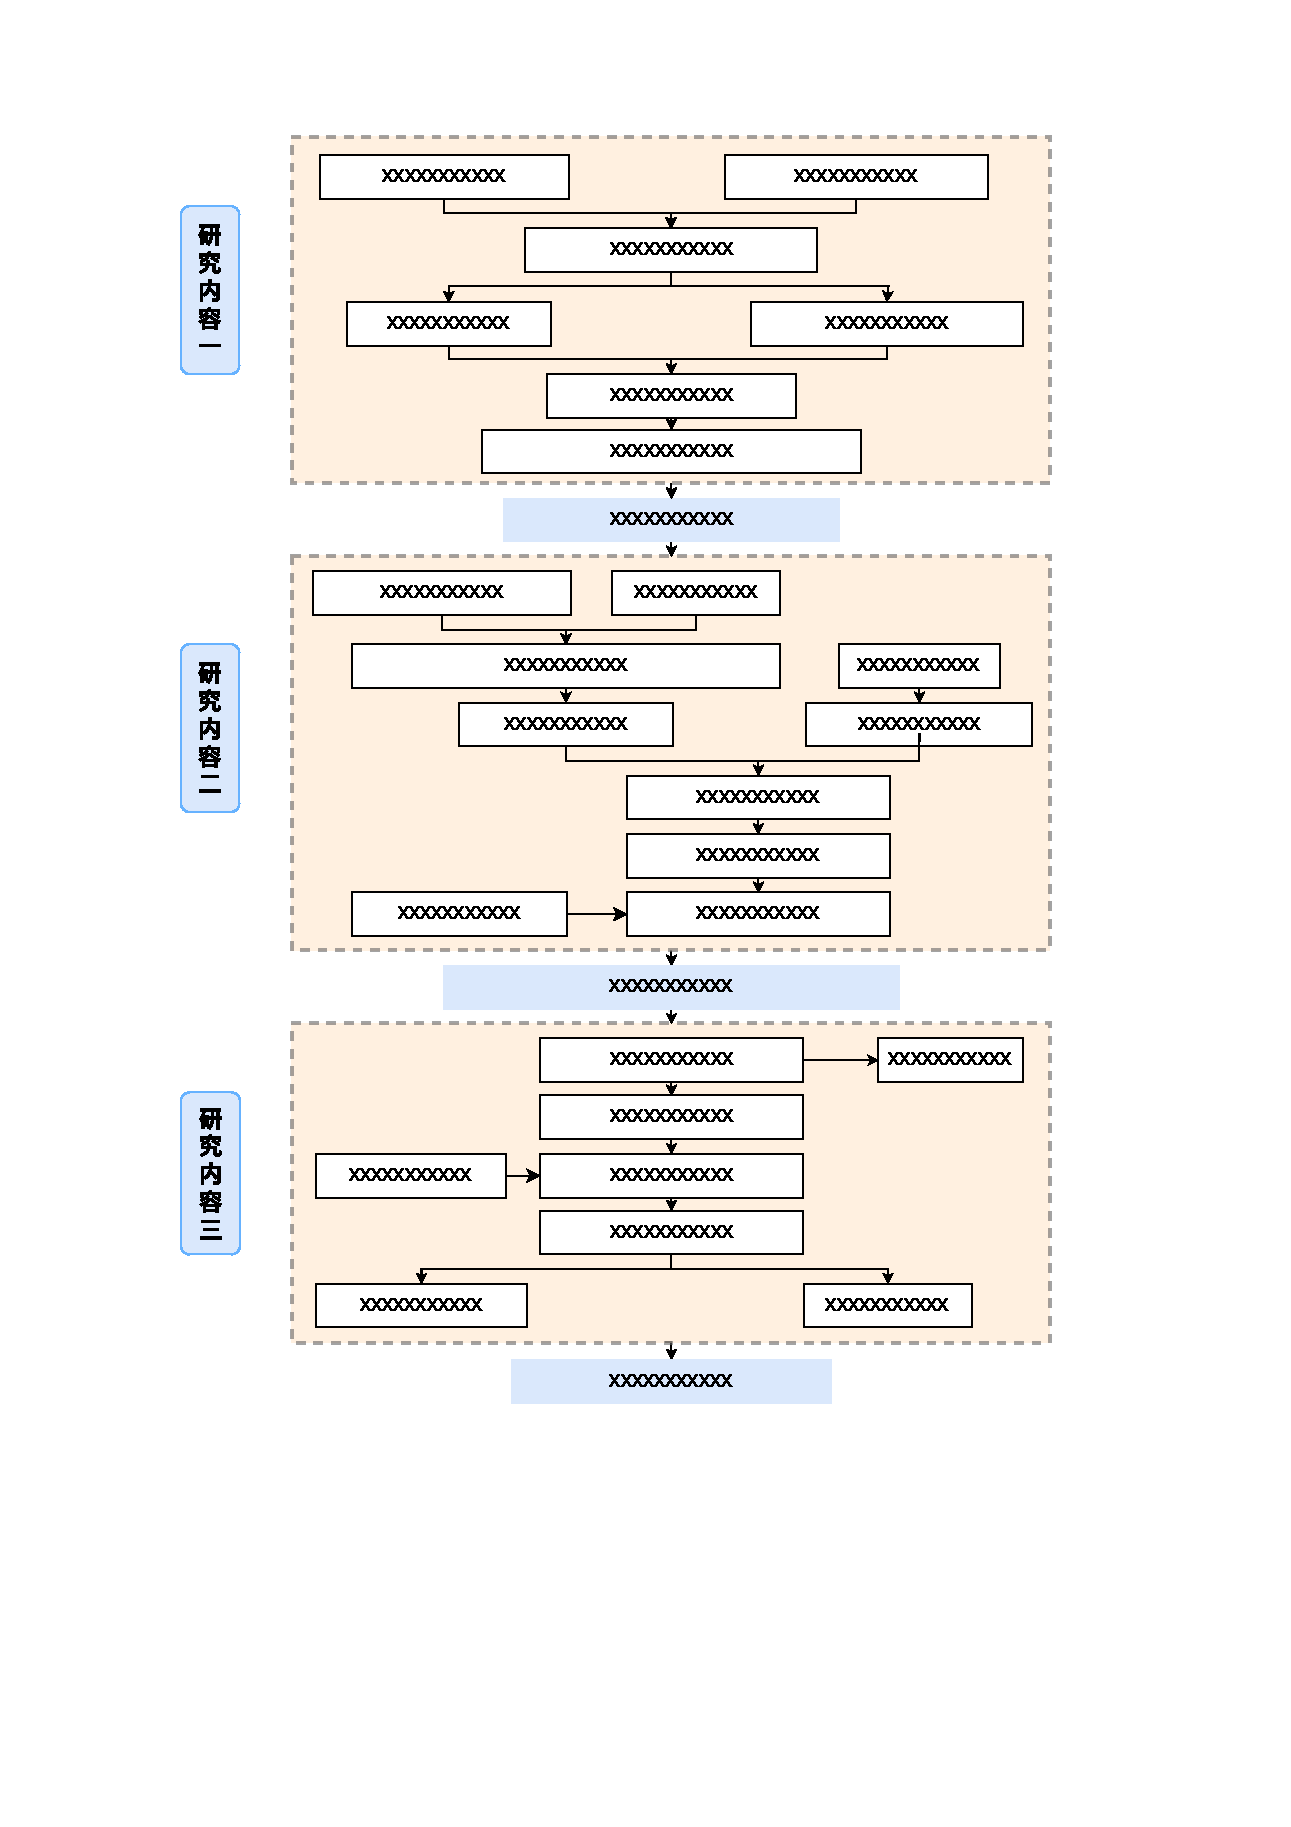
\includegraphics[width=0.95\columnwidth]{figures/roadmap.pdf}
	\caption{总体技术路线图\label{fig:roadmap}}
\end{figure}


\subsection{关键技术}

\subsubsection*{(1) 关键技术一}

\subsubsection*{(2) 关键技术二}

\subsubsection*{(3) 关键技术三}

\subsection{可行性分析}

\subsubsection*{(1) 研究方案原理层面的可行性}

申请人此前在XXX方面积累了丰富的研究经验,证明了XXX,研究成果已发表在\journal{XXX Journal} (2024, 1(1), 1-10)、\journal{XXX Journal} (2024, In press, DOI: XXX)等期刊上(\alert{详见研究基础“XXX”部分})。

\subsubsection*{(2) 研究方案技术路线层面的可行性}

\textbf{1) 研究内容一的可行性}

\textbf{2) 研究内容二的可行性}

\textbf{3) 研究内容三的可行性}

\subsubsection*{(3) 研究方案实施层面的可行性}

\NsfcSection{4}{本项目的特色与创新之处;}{}

\subsubsection*{(1) 理论模型创新}

\subsubsection*{(2) 研究方法创新}

\NsfcSection{5}{年度研究计划及预期研究结果}{
(包括拟组织的重要学术交流活动、国际合作与交流计划等)。}

\subsection{年度研究计划}

本项目执行期三年(20XX.01\textasciitilde 20XX.12),具体年度计划如下:
\begin{sloppypar}
	\begin{itemize}[itemindent=6.5pt]
		\item[$\blacksquare$] \textbf{第一年度(20XX.01\textasciitilde 20XX.12)}
			\begin{enumerate}[label=\arabic*)]
				\item 完成XXX;
				\item 完成XXX;
				\item 完成XXX。
			\end{enumerate}
		\item[$\blacksquare$] \textbf{第二年度(20XX.01\textasciitilde 20XX.12)}
			\begin{enumerate}[label=\arabic*)]
				\item 完成XXX;
				\item 完成XXX;
				\item 完成XXX。
			\end{enumerate}
		\item[$\blacksquare$] \textbf{第三年度(20XX.01\textasciitilde 20XX.12)}
			\begin{enumerate}[label=\arabic*)]
				\item 完成XXX;
				\item 完成XXX;
				\item 完成XXX。
			\end{enumerate}	
	\end{itemize}
\end{sloppypar}


\subsection{预期研究成果}
本项目预计取得的成果如下:
\begin{enumerate}[label=\arabic*)]
	\item 完成XXX;
	\item 完成XXX;
	\item 在高水平学术期刊发表学术论文X\textasciitilde X篇;申请国家发明专利X\textasciitilde X项。
\end{enumerate}

%%%%%%%%%%%%%%%%%%%%%%%%%%%%%%%%%%%%%%%%%%%%%%%%%
\ContentDes{(二)研究基础与工作条件}{}

\NsfcSection{1}{研究基础}{
(与本项目相关的研究工作积累和已取得的研究工作成绩);}

申请人简介。

\subsection{相关工作积累}

\subsubsection*{(1) XXX的前期研究}

\subsubsection*{(2) XXX的前期研究}

\subsubsection*{(3) XXX的前期研究}

\subsubsection*{(4) XXX的前期研究}

\subsection{代表性成果}

\noindent\textbf{(1) 学术期刊论文}
\begin{sloppypar}
	\small
	\begin{enumerate}[align=right, labelindent=0pt, itemindent=0pt, leftmargin=\parindent]
            \item \authorFormat{San Zhang (独立一作)}, Si Li, Wu Wang, et al., XXX research paper, \journal{XXX journal}, 2024, 1(1): 1-10 (中科院1区, Top).
            \item \authorFormat{San Zhang (独立一作)}, Si Li, Wu Wang, et al., XXX research paper, \journal{XXX journal}, 2024, 1(1): 1-10 (中科院2区, Top).
            \item \authorFormat{San Zhang (独立一作)}, Si Li, Wu Wang, et al., XXX research paper, \journal{XXX journal}, 2024, 1(1): 1-10 (中科院3区).
            \item Si Li\dag, \authorFormat{San Zhang\dag (共同一作)},  Wu Wang, et al., XXX research paper, \journal{XXX journal}, 2024, 2(1): 1-10 (中科院2区).  
            \item Si Li, Wu Wang, Liu Zhao, \authorFormat{San Zhang* (唯一通讯)}., XXX research paper, \journal{XXX journal}, 2024, 3(1): 1-10 (中科院3区).
            \item Si Li, \authorFormat{San Zhang (学生一作)},  Wu Wang, et al., XXX research paper, \journal{XXX journal}, 2024, 1(1): 1-10 (中科院1区, Top).
	\end{enumerate}
\end{sloppypar}

\noindent\textbf{(2) 国家发明专利}
\begin{sloppypar}
	\small
	\begin{enumerate}[align=right, labelindent=0pt, itemindent=0pt, leftmargin=\parindent]
		\item \authorFormat{张三}, 李四, 王五, 等, 某发明专利, ZLXXXXXXXXX.X, 授权日期: 2024-01-01.
  		\item 李四, \authorFormat{张三}, 王五, 等, 某发明专利, ZLXXXXXXXXX.X, 授权日期: 2024-01-01.
		\item \authorFormat{张三}, 李四, 王五, 等, 某发明专利, CNXXXXXXXXX.X, 申请日期: 2024-01-01.
  		\item \authorFormat{张三}, 李四, 王五, 等, 某发明专利, CNXXXXXXXXX.X, 申请日期: 2024-01-01.
		\item \authorFormat{张三}, 李四, 王五, 等, 某发明专利, CNXXXXXXXXX.X, 申请日期: 2024-01-01.
	\end{enumerate}
\end{sloppypar}

\NsfcSection{2}{工作条件}{
(包括已具备的实验条件,尚缺少的实验条件和拟解决的途径,包括利用国家实验室、国家重点实验室和部门重点实验室等研究基地的计划与落实情况);}

Lorem Ipsum是一种常用的虚拟填充文本,在网页设计和排版领域有着广泛的应用。它的历史可以追溯到16世纪,最初被用作印刷业的占位符文本。Lorem Ipsum文本并非无意义的乱码,而是源自古罗马时期的拉丁文文献。经过几个世纪的发展,这段文本逐渐演变成了一种标准化的虚拟填充文本,被广泛应用于各种设计项目中。

Lorem Ipsum之所以能够经久不衰,一方面是因为其本身的可读性和连贯性,另一方面则得益于它能够有效地模拟真实文本的视觉效果,帮助设计师们更好地预览最终的设计成果。随着数字时代的发展,Lorem Ipsum也逐渐从传统的印刷领域扩展到了网页设计、移动应用等多个领域,成为了设计师们不可或缺的工具之一。生能够将主要精力用于此项目的研究工作,确保此课题按期、保质、保量完成。

\NsfcSection{3}{正在承担的与本项目相关的科研项目情况}{
(申请人正在承担的与本项目相关的科研项目情况,包括国家自然科学基金的项目和国家其他科技计划项目,要注明项目的资助机构、项目类别、批准号、项目名称、获资助金额、起止年月、与本项目的关系及负责的内容等);}

无

\NsfcSection{4}{完成国家自然科学基金项目情况}{(对申请人负责的前一个已资助期满的科学基金项目(项目名称及批准号)完成情况、后续研究进展及与本申请项目的关系加以详细说明。另附该项目的研究工作总结摘要(限500字)和相关成果详细目录)。}

无

%%%%%%%%%%%%%%%%%%%%%%%%%%%%%%%%%%%%%%%%%%%%%%%%%
\ContentDes{(三)其他需要说明的情况}{}

\NsfcSection{1}{}{申请人同年申请不同类型的国家自然科学基金项目情况(列明同年申请的其他项目的项目类型、项目名称信息,并说明与本项目之间的区别与联系)。}

无

\NsfcSection{2}{}{具有高级专业技术职务(职称)的申请人是否存在同年申请或者参与申请国家自然科学基金项目的单位不一致的情况;如存在上述情况,列明所涉及人员的姓名,申请或参与申请的其他项目的项目类型、项目名称、单位名称、上述人员在该项目中是申请人还是参与者,并说明单位不一致原因。}

无

\NsfcSection{3}{}{具有高级专业技术职务(职称)的申请人是否存在与正在承担的国家自然科学基金项目的单位不一致的情况;如存在上述情况,列明所涉及人员的姓名,正在承担项目的批准号、项目类型、项目名称、单位名称、起止年月,并说明单位不一致原因。}

无

\NsfcSection{4}{}{其他。}

无

\end{document}
